\documentclass[../../main.tex]{subfiles}
\begin{document}
This section will introduce the tests prompted by the requirements in section \ref{sec:Requirements} and present the results. These results will determine whether it has been possible to comply with the requirement specifications. Additional data from the tests can be seen in the digital appendix. 

To ease access to data from the FPGA during tests, a \textit{microblaze} has been implemented, which utilises UART to communicate directly with a computer. This allows for direct access to the position and velocity of the pan and tilt motor making data processing easier. 

\subsection{Microcontroller Timing Test}
Running multiple tasks on one microcontroller it is imperative to know, how much of the CPU time is utilised. If the CPU is overloaded the risk of starvation is introduced. In addition it is wanted to examine the processing time of the controllers on the microcontroller, to be able to deduce the overhead, thus it is wanted to test whether the system can satisfy the requirement from section \ref{sec:Requirements}:
\begin{itemize}
    \item The PID-controllers must not utilize more than \SI{60}{\percent} of the CPU time on the microcontroller.
    \item It must be verified that the overhead does not compromise the timing of the system.
    \item A maximum execution time for the PID-controller must be determined.
\end{itemize}

To estimate a maximum allowed processing time for a controller, the maximum time for which the PID-controllers may utilise the CPU time is divided into four parts. With a maximum CPU time utilisation of \SI{60}{\percent}, a single controller is to be processed within $\SI{150}{\micro \second}$.

The single controller test is performed with the velocity controller described in section \ref{sec:System_Integration_N_Implementation} using a fifth order derivative filter. The CPU utilisation test is executed with four controllers, the UART task and the SPI task running with FreeRTOS. The UI task is not taken into account, because no user input is required for the test. The position controllers are scheduled at a frequency of \SI{200}{\hertz} and the velocity controllers at \SI{1000}{\hertz}. The timing of the tasks are done by driving pins high upon start and low upon end of the task cycle of all individual tasks, thus enabling the possibility of timing the tasks with an oscilloscope.


\subsubsection*{Results}
Table \ref{tab:CPU_utilisation_test} shows the timing of running the controllers including the UART, SPI and UI task. 
$t_1$ is the duration of two velocity PID-controller tasks and $t_2$ is the duration of two position PID-controllers tasks. $T_ce$ is the duration between the first task starts to the same task starts again, as seen on figure \ref{fig:Schedueling_controllers}. This makes it possible to estimate the average CPU utilisation of the PID-controller tasks as seen in equation \ref{eq:CPU_util},
\begin{equation}\label{eq:CPU_util}
    U_{CPU} =\left(\frac{t_{1,avg} + t_{2,avg}}{T_{c,avg}}\right)\cdot 100=\left(\frac{\SI{457,6}{\mu\second}}{\SI{992}{\mu\second}}\right)\cdot 100\approx \SI{46,13}{\percent}
\end{equation}
where $ U_{CPU,avg} $ is the average CPU utilisation, $t_{1,avg}$ and $ t_{2,avg}$ is the average duration of $t_1$ and $t_2$ and $T_{c,avg}$ is the average time of $T_c$ as seen on figure \ref{fig:Schedueling_controllers}. 

\begin{table}[H]
\centering
\begin{tabular}{lrrrrr}
\multicolumn{1}{c}{\textbf{}}            & \multicolumn{5}{c}{\textbf{Test number}}                                                                                              \\
\multicolumn{1}{r|}{}                    & \multicolumn{1}{r|}{1}    & \multicolumn{1}{r|}{2}    & \multicolumn{1}{r|}{3}    & \multicolumn{1}{r|}{4}    & \multicolumn{1}{r}{5} \\ \hline
\multicolumn{1}{l|}{$t_1 + t_2$ (\SI{}{\micro\second})} & \multicolumn{1}{r|}{458}  & \multicolumn{1}{r|}{456}  & \multicolumn{1}{r|}{456}  & \multicolumn{1}{r|}{460}  & 458                   \\
\multicolumn{1}{l|}{$T_c$ (\SI{}{\micro\second})}                 & \multicolumn{1}{r|}{990}  & \multicolumn{1}{r|}{988}  & \multicolumn{1}{r|}{994}  & \multicolumn{1}{r|}{994}  & 994                   \\
\multicolumn{1}{l|}{$U_{CPU}$ (\SI{}{\percent})}          & \multicolumn{1}{r|}{46,3} & \multicolumn{1}{r|}{46,1} & \multicolumn{1}{r|}{45,9} & \multicolumn{1}{r|}{46,3} & 46,1                 
\end{tabular}
\caption{Data regarding the duty cycle of the controller process scheduled with two position and two velocity controllers, the UART and SPI task. The position controllers, $t_2$ are scheduled at a rate of \SI{200}{\hertz} and the velocity controllers, $t_1$ at \SI{1000}{\hertz}. Figure \ref{fig:Schedueling_controllers} illustrates the test.}
\label{tab:CPU_utilisation_test}
\end{table}

% Please add the following required packages to your document preamble:
% \usepackage{graphicx}
% Please add the following required packages to your document preamble:
% \usepackage{graphicx}
\begin{table}[H]
\centering
\begin{tabular}{lrrrrr}
\multicolumn{1}{c}{\textbf{}}            & \multicolumn{5}{c}{\textbf{Test number}}                                                                                                 \\
\multicolumn{1}{l|}{}                    & \multicolumn{1}{r|}{1}     & \multicolumn{1}{r|}{2}     & \multicolumn{1}{r|}{3}    & \multicolumn{1}{r|}{4}     & \multicolumn{1}{r}{5} \\ \hline
\multicolumn{1}{l|}{SPI\_transmit (\SI{}{\micro\second})}       & \multicolumn{1}{r|}{9,9}   & \multicolumn{1}{r|}{9,75}  & \multicolumn{1}{r|}{9,75} & \multicolumn{1}{r|}{9,74}  & 9,75                  \\
\multicolumn{1}{l|}{SPI\_receive (\SI{}{\micro\second})}        & \multicolumn{1}{r|}{5,44}  & \multicolumn{1}{r|}{5,44}  & \multicolumn{1}{r|}{5,44} & \multicolumn{1}{r|}{5,46}  & 5,45                  \\
\multicolumn{1}{l|}{UART (\SI{}{\nano\second})}                & \multicolumn{1}{r|}{458}   & \multicolumn{1}{r|}{500}   & \multicolumn{1}{r|}{500}  & \multicolumn{1}{r|}{500}   & 501                   \\
\multicolumn{1}{l|}{Velocity Controller (\SI{}{\micro\second})} & \multicolumn{1}{r|}{107,8} & \multicolumn{1}{r|}{107,8} & \multicolumn{1}{r|}{108}  & \multicolumn{1}{r|}{107,8} & 107,8                
\end{tabular}
\caption{Timing of SPI upon transmission and receiving, the UART task and velocity PID-controller.}
\label{tab:Task_Timing}
\end{table}

Table \ref{tab:Task_Timing} shows the timing of the UART, SPI and the velocity PID-controller task respectively. As seen in the table, the PID-controller has an average processing time of $\SI{107,8}{\micro \second}$ with an fifth order derivative filter. In accordance with the requirement specification this is sufficient for a single controller.
\begin{figure}
    \centering
    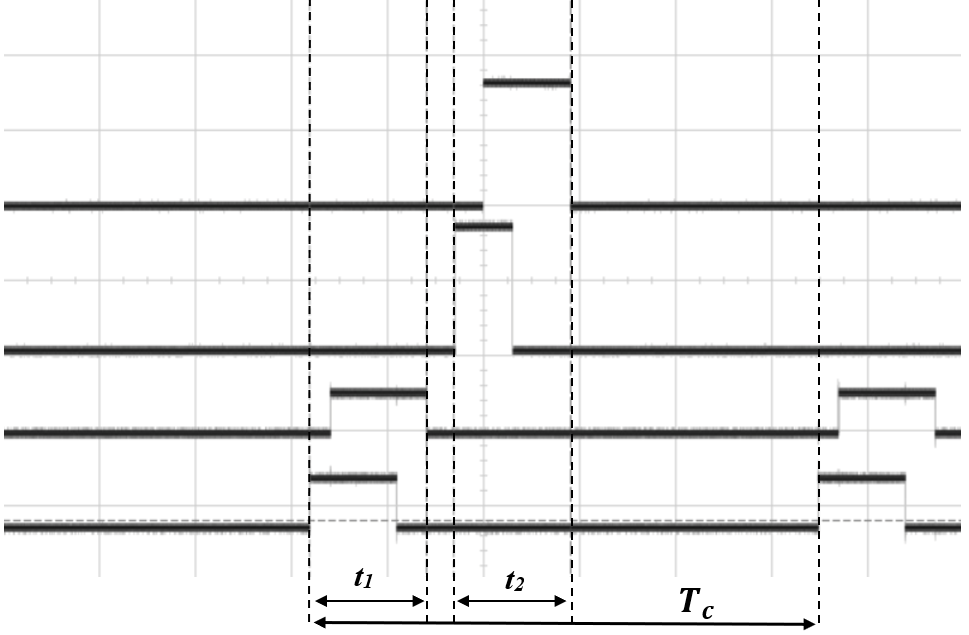
\includegraphics[width=0.7\textwidth]{Sections/Test/Images/TestMicrocontrollerTiming.png}
    \caption{Illustration of the scheduling of the four controllers running with two position and two velocity controllers, the UART, SPI and UI task.
    
    $t_2$ are the position controllers run at a rate of \SI{200}{\hertz}.$t_1$ are the velocity controllers run at a rate of \SI{1000}{\hertz}.}
    \label{fig:Schedueling_controllers}
\end{figure}

However it is also possible to get an estimation of the overhead of the system by comparing the values of table \ref{tab:Task_Timing} and \ref{tab:CPU_utilisation_test}. This is done by comparing the total time of executing four PID-controllers and the time of processing a single PID-controller as seen in equation \ref{eq:overhead},

\begin{equation}\label{eq:overhead}
    \mathrm{overhead}=\frac{T_{c}-(T_{controller}\cdot 4)}{T_{c1}}\cdot 100 \approx \SI{5,7}{\percent} \qquad ,
\end{equation}
where $T_{controller}$ is the processing time of a single velocity controller.

%%%%%-----


  %It was however desired to test the influence of the derivative term and the additional filter on the derivative term. According to the test, the derivative term as implemented in the project adds an average of $\SI{16,68}{\mu\second}$ to the processing time.

% \begin{table}[H]
% \begin{tabular}{l|c|r|r|r|r|r}
% \textbf{Controller (Velocity)} & \multicolumn{1}{l|}{\textbf{Filter order}} & \textbf{1} & \textbf{2} & \textbf{3} & \textbf{4} & \multicolumn{1}{r|}{\textbf{5}}                                   \\ \hline
% PID-controller (\SI{}{\mu\second})                   & 4                                 & 104,4 & 104,4 & 104,6 & 104,6 & \multicolumn{1}{r|}{117,8}       \\
% - (\SI{}{\mu\second})  & 6                                 & 107,8 & 107,8 & 108   & 107,8 & \multicolumn{1}{r|}{108}           \\
% - (\SI{}{\mu\second})           & 8                                 & 111,2 & 111   & 110,8 & 111,2 & \multicolumn{1}{r|}{111,2}        \\
% % PID without filter                & -                                 & 95,2  & 95,6  & 94,6  & 94,2  & \multicolumn{1}{r|}{95,2}  & \SI{}{\mu\second}        \\
% % PI without D-term                 & -                                 & 94,4  & 94,4  & 94,6  & 94,2  & 94,4                       & \SI{}{\mu\second}     
% \end{tabular}
% \caption{Data regarding the duration of processing the position controller. The filter order is regarding the filter filtering the derivative term of the controller. All tests are made with a third order filter for the input.}
% \label{tab:Single_Controller_test}
% \end{table}


\subsection{SPI Stress Test}
Using SPI as the only communication between the FPGA and the microcontroller, it is essential to test the reliability of the system to ensure that no information is lost during transmission. 
\begin{itemize}
    \item Using SPI with a bit rate of \SI{13,3}{\mega bit}, the FPGA is to receive \SI{99,9}{\percent} messages correct with no errors.
\end{itemize}
The test was preformed by sending 10000 messages from the microcontroller to the FPGA. Each message contains the value of a counter, starting at 0 and incrementing to 9999. Subsequent is each message transmitted to a computer with the help of the microblaze, and processed to check if all values are present and in the correct sequence.  

\begin{table}[]
    \centering
    \begin{tabular}{L{1.4 cm} | c{5 cm} c{3 cm} c{3 cm} 
         \textbf{Test number} & \textbf{Transmission Rate [\si{\kilo\hertz}]} & \textbf{Messages sent} & \textbf{Messages Received}  \\
         \hline
         1 & 1 & 1 & 1 \\
         1 & 1 & 1 & 1 \\
         1 & 1 & 1 & 1 \\
         1 & 1 & 1 & 1 \\
         1 & 1 & 1 & 1 
    \end{tabular}
    \caption{Caption}
    \label{tab:my_label}
\end{table}


\begin{table}[H]
\centering
\begin{tabular}{c|c|c|c}
Test no. & Transmission Rate {[}kHz{]} & Msg. sent & Msg. received \\ \hline
1-5 & 2 & 10000 & 10000
\end{tabular}
\caption{Data regarding the five test performed with SPI.}
\label{tab:SPI-stresstest}
\end{table}

As seen in table \ref{tab:SPI-stresstest} the five test resulted in the same outcome, with all messages being received and in the correct sequence. 

\subsection{Test of Controller Designs}\label{subsec:testControllerDesign}
%opdeling af afsnit
This section concerns the test of the PID-controllers using different methods for tuning and designs. The parameters used in each test is shown in table \ref{tab:pos_controller_gains}, and are designed using the design guides of \SI{5}{\percent} overshoot, \SI{1,5}{\second} settling time and \SI{0,5}{\second} rise time as described in section \ref{sec:System_Design}.
% \begin{table}[H]
% \centering
% \begin{tabular}{c|c|c|c|c|c|c|c|c|}
%       & \multicolumn{2}{l|}{Position Controllers} & \multicolumn{2}{l|}{Velocity Controller (tilt)} & \multicolumn{4}{c|}{Cascade Controller (tilt)}                                                                                                                                                                                \\ \hline
%       & Tilt                & Pan                 & ZN                      & PP                    & \begin{tabular}[c]{@{}c@{}}ZN\\ Position\end{tabular} & \begin{tabular}[c]{@{}c@{}}ZN\\ Velocity\end{tabular} & \begin{tabular}[c]{@{}c@{}}PP\\ Position\end{tabular} & \begin{tabular}[c]{@{}c@{}}PP\\ Velocity\end{tabular} \\
% $k_P$ & 9.450               & 4.920               & 0.519                   & 1.422                 & 8.740                                                 & 0.519                                                 & 7.528                                                 & 1.420                                                 \\ 
% $k_I$ & 8.550               & 3.170               & 22.860                  & 7.800                 & 7.640                                                 & 22.860                                                & 7.589                                                 & 7.800                                                 \\ 
% $k_D$ & 0.900               & 1.200               & 0.003                   & 0.065                 & 1.220                                                 & 0.003                                                 & 1.030                                                 & 0.065                                                 \\ 
% \end{tabular}
% \caption{Parameters used for each test. ZN is deduced using the Zielger-Nichols method and PP is deduced using pole placement.}
% \label{tab:TestParameters}
% \end{table}

%Test metoden
\subsubsection*{Single Position Controller using Pole Placement}

\begin{figure}[h]
     \centering
     \begin{subfigure}[b]{0.49\textwidth}
         \centering
         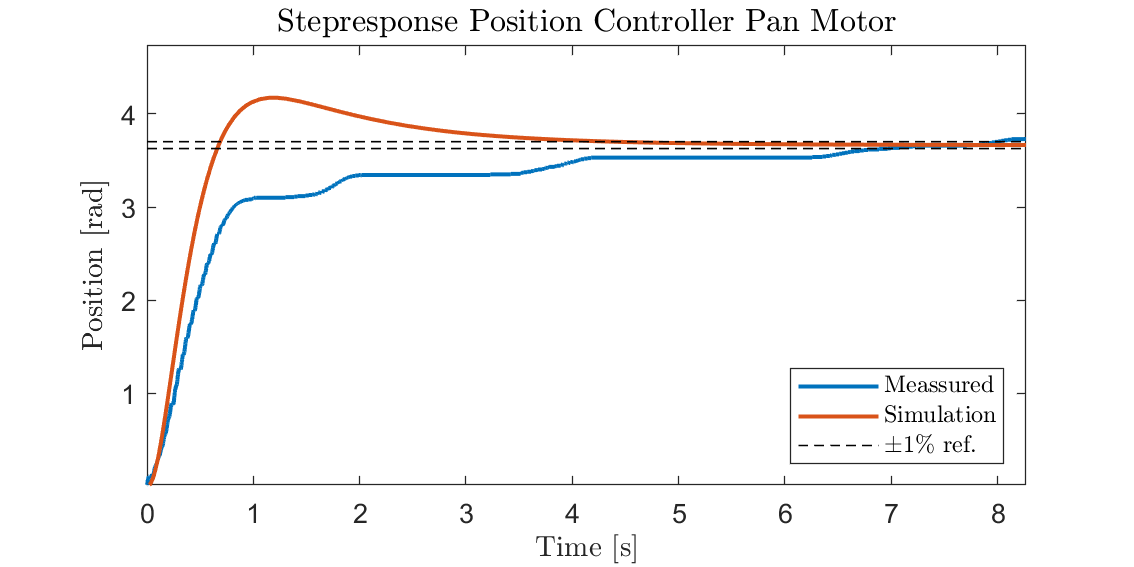
\includegraphics[width=\textwidth]{Sections/Test/Images/StepPanPosModel.png}
         \caption{Pan motor}
         \label{fig:StepPanPos}
     \end{subfigure}
     \hfill
     \begin{subfigure}[b]{0.49\textwidth}
         \centering
         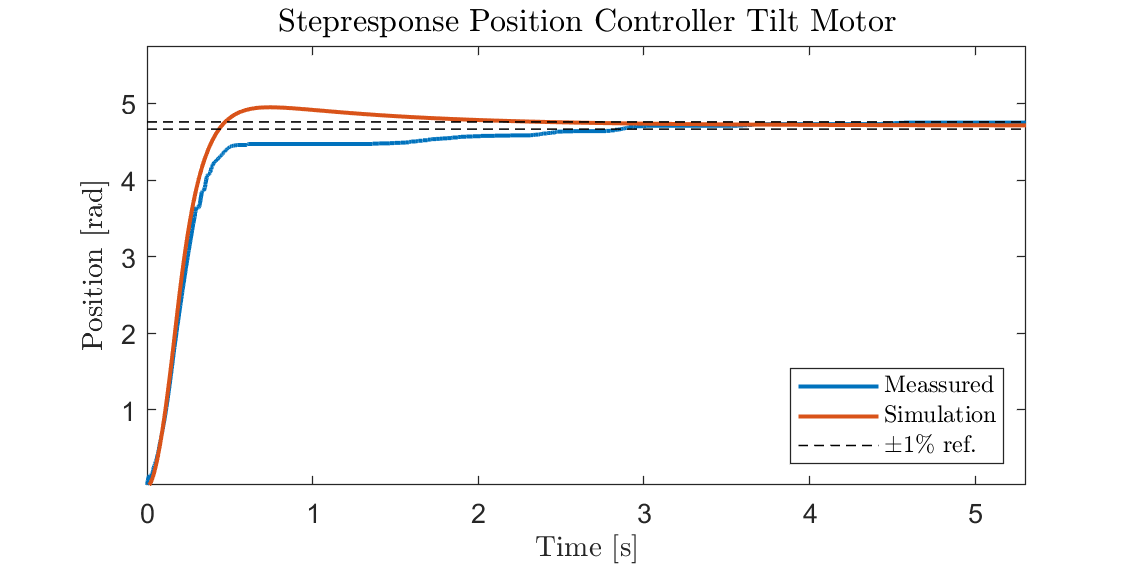
\includegraphics[width=\textwidth]{Sections/Test/Images/StepTiltPosModel.png}
         \caption{Tilt motor}
         \label{fig:StepTiltPos}
     \end{subfigure}
        \caption{Step response of the position using a single controller with pole placement. The measured response being an average of five tests.}
        \label{fig:singlePosController}
\end{figure}
The tests are executed with a reference point of $\theta = \frac{7\pi}{6}\SI{}{\radian}$ for the pan motor and $\theta = \frac{3\pi}{2}\SI{}{\radian}$. As seen on figure \ref{fig:StepPanPos} the measured response has a slower step response compared to the simulated. Furthermore there are stationary points in the measured response, showing that the pan frame has stopped moving. On figure \ref{fig:StepTiltPos} the measured response resembles the simulated quite well. The data for the tests can be seen on table \ref{tab:controller_data}. Applicable for both measurements is that they have no overshoot and longer settling times than the simulated. 


\subsubsection*{Velocity Controller for the Tilt Motor}
The velocity controller is tested using gains found from the Ziegler-Nichols and pole placement methods on the tilt motor. A reference point of $\Dot{\theta}=\SI{20}{\radian \per \second}$ is used. As seen on figure \ref{fig:StepVelZN} the measured response initially resembles the simulated signal using the Ziegler-Nichols method. Seen on figure \ref{fig:StepVelModel}, using pole placement a very slow response compared to the simulated is achieved in addition to a steady state error. Studying data from figure \ref{fig:StepVelZN} further it appears like a small steady state error is present as well. The reason for this behaviour is discussed in section \ref{sec:Discussion}. Applicable for both tests are that the measured signal is corrupted by noise. Data regarding the performance of the controllers are presented in table \ref{tab:controller_data}.

\begin{figure}[h]
     \centering
     \begin{subfigure}[b]{0.49\textwidth}
         \centering
         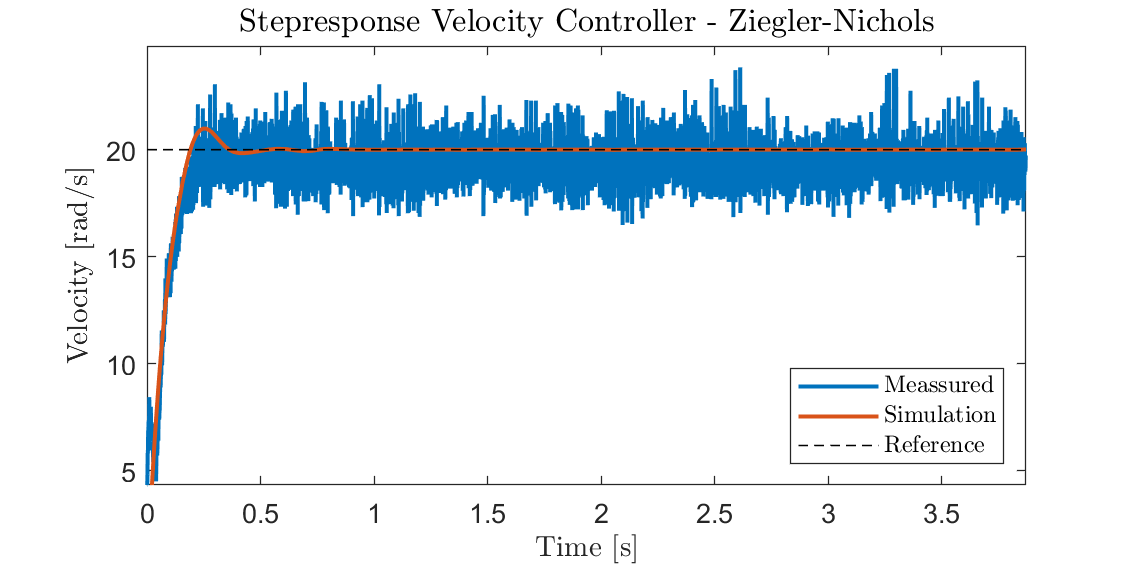
\includegraphics[width=\textwidth]{Sections/Test/Images/StepVelocityZN.png}
         \caption{Ziegler-Nichols}
         \label{fig:StepVelZN}
     \end{subfigure}
     \hfill
     \begin{subfigure}[b]{0.49\textwidth}
         \centering
         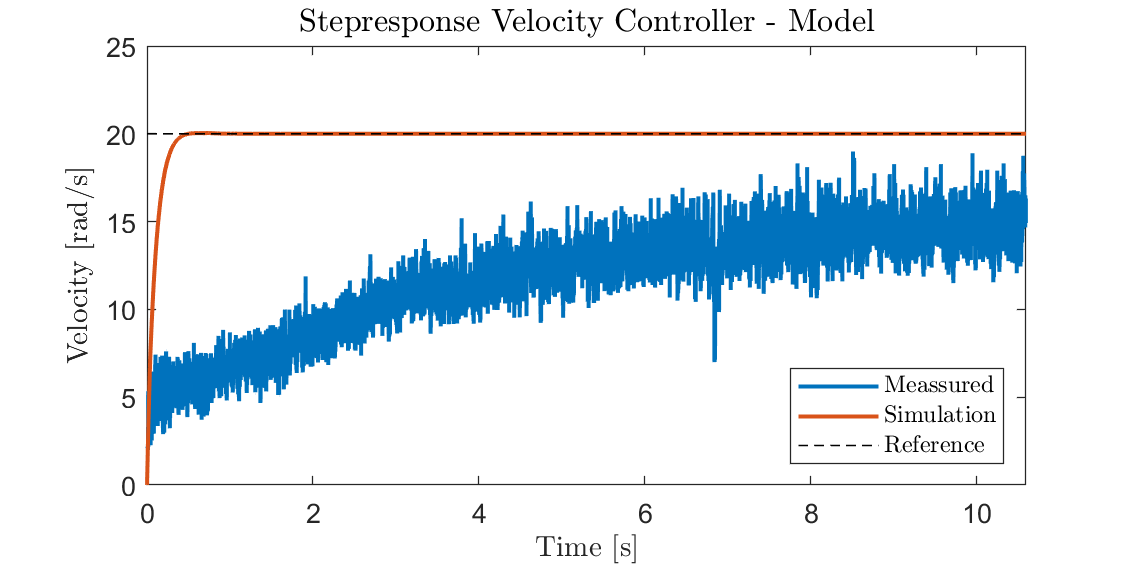
\includegraphics[width=\textwidth]{Sections/Test/Images/StepVelocityModel.png}
         \caption{Pole Placement}
         \label{fig:StepVelModel}
     \end{subfigure}
        \caption{Step response of a single velocity controller on the tilt motor. The measured response being an average of five tests.}
        \label{fig:VelocityTilt}
\end{figure}

\subsubsection*{Cascaded Position Controller for the Tilt Motor}
The cascaded PID-controller design is tested using the velocity controller gains analysed above and the position controller gains found using the pole placement method based on the velocity controllers. A reference point of $\theta = \frac{3\pi}{2} \SI{}{\radian}$ is used. Figure \ref{fig:Cascade_ZN_tilt} shows that using the Ziegler-Nichols method, the measured signal resembles the simulated response quite well. However using the pole placement method, illustrated on figure \ref{fig:cascade_model_tilt}, the measured response has a lot more overshoot than the simulated response. It could appear that this is due to the poor velocity response, which is discussed in section \ref{sec:Discussion}. The performance results are presented in table \ref{tab:controller_data}.

\begin{figure}[h]
     \centering
     \begin{subfigure}[b]{0.49\textwidth}
         \centering
         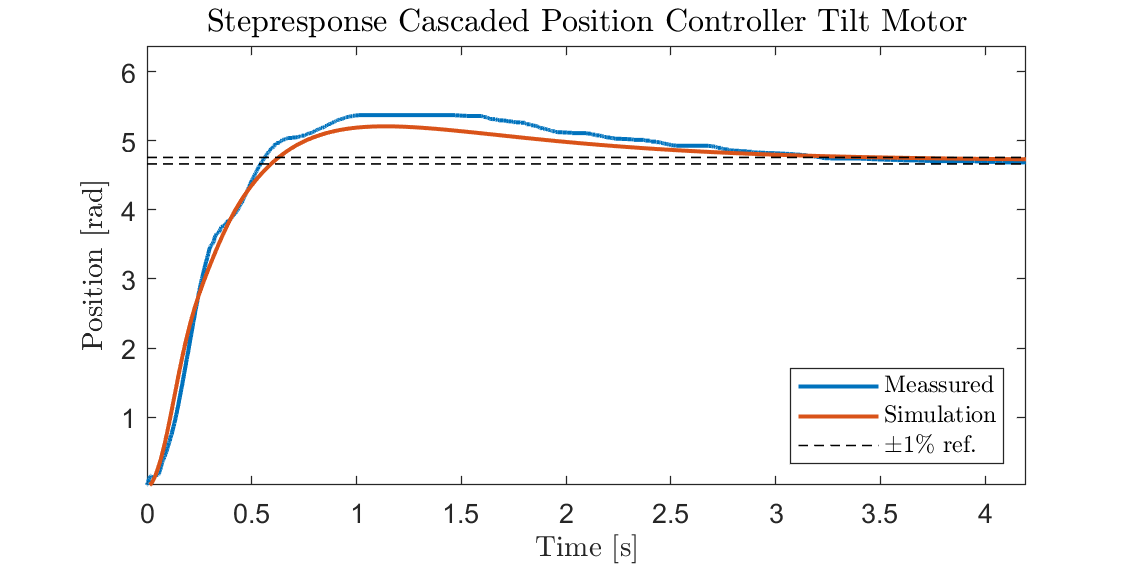
\includegraphics[width=\textwidth]{Sections/Test/Images/cascade_ZN_tilt.png}
         \caption{Ziegler-Nichols method}
         \label{fig:Cascade_ZN_tilt}
     \end{subfigure}
     \hfill
     \begin{subfigure}[b]{0.49\textwidth}
         \centering
         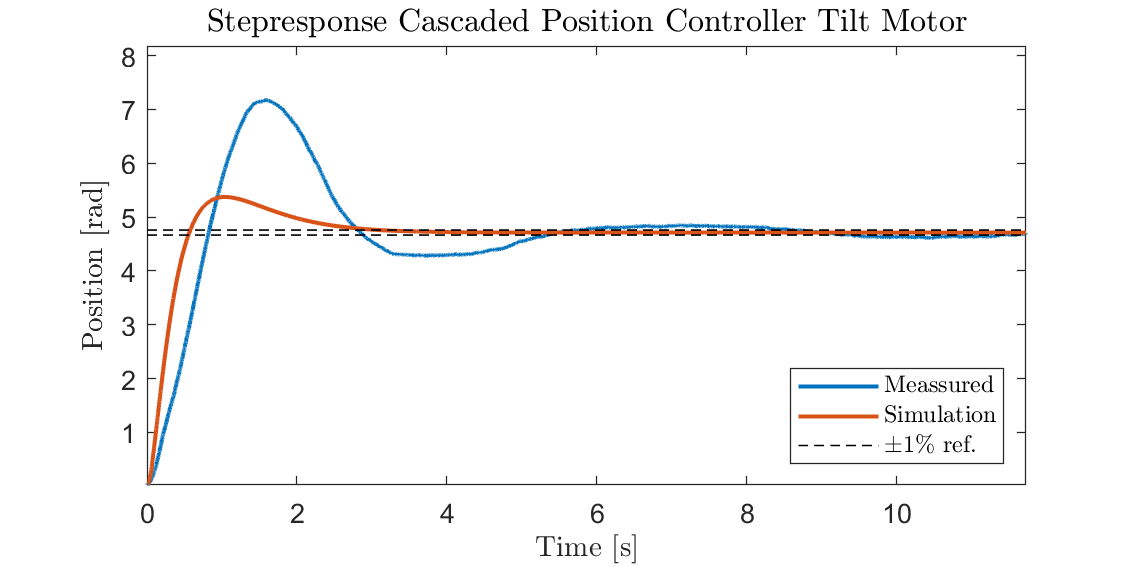
\includegraphics[width=\textwidth]{Sections/Test/Images/cascade_Model_tilt.png}
         \caption{Pole Placement method}
         \label{fig:cascade_model_tilt}
     \end{subfigure}
        \caption{Step response of a cascaded PID-controller for the position of the tilt motor. The measured response being an average of five tests.}
        \label{fig:CascadeTilt}
\end{figure}

\subsubsection*{Cascaded Position Controller for the Pan Motor}
The cascaded controller on the pan motor is executed using a reference point of $\theta = \frac{7\pi}{6}$. Since no cascaded controller has been designed for the pan motor, the parameters are identical with the ones used for the cascaded tilt controller based on the Ziegler-Nichols method. This is done mainly as means to evaluate the accuracy of the pan motor model, by comparing the measured response with the simulated response. But also to assess the importance of customising the gains for the specific motor.
According to figure \ref{fig:cascade_ZN_pan}, the measured signal seems to have a slower response than the simulated response. However neither the simulated nor the measured response are considered ideal, which highlights the importance of tailoring the gains for the specific motor.

\begin{figure}[h]
    \centering
    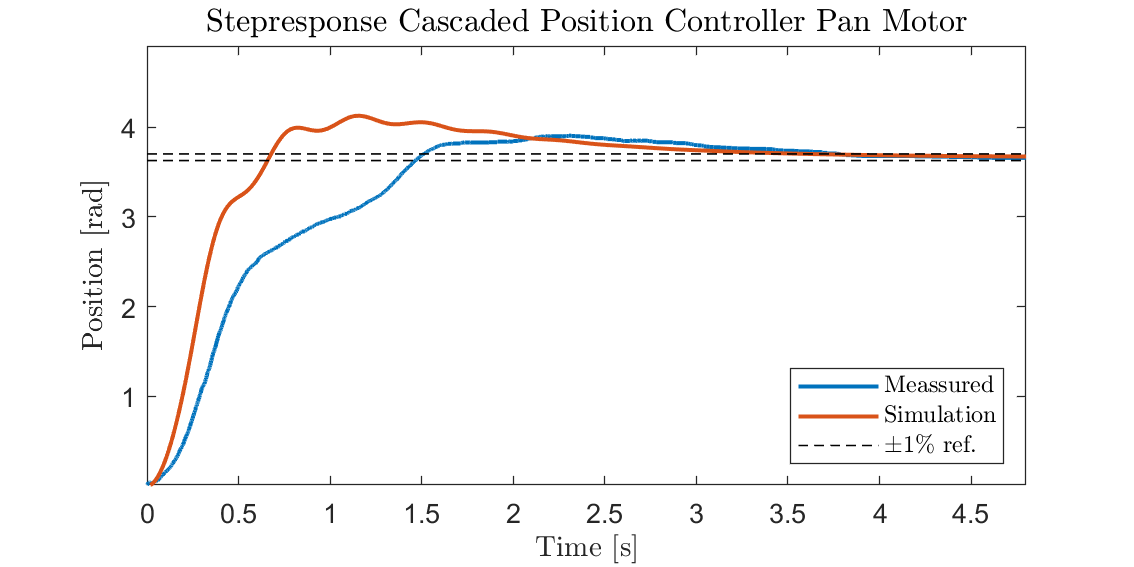
\includegraphics[width = 0.7 \textwidth]{Sections/Test/Images/cascade_ZN_pan.png}
    \caption{Position step response using a cascaded PID-controller for the pan motor. The measured response being an average of five tests.}
    \label{fig:cascade_ZN_pan}
\end{figure}

\subsubsection*{Results}
Table \ref{tab:controller_data} shows the data regarding the performance of the different PID-controllers. As it is seen none of the designed controllers satisfies the specifications of less than \SI{5}{\percent} overshoot, \SI{1,5}{\second} settling time and \SI{0,5}{\second} rise time, however some controllers achieved better results than others. The single position PID-controller seems to have the overall best performance in relation the the requirement specifications. The reason for the deviations comparing the simulation and the measured are discussed in section \ref{sec:Discussion}.
\begin{table}[H]
    \centering
    \begin{tabular}{c|c|c|c|c|c}
         Controller & Motor & Method & Overshoot (\%) & Settling Time (s)  & Rise Time (s) \\ \hline
         Position & Pan & Pole placement & 14.3 & 8.27 & 1.74  \\
         Position & Tilt & Pole placement & 0.8 & 2.86 & 0.34  \\
         Velocity & Tilt & Ziegler-Nichols & 19.2 & N/A & 0.15  \\
         Velocity &Tilt & Pole placement & N/A & N/A & 7.8 \\
         Cascade & Tilt  & Pole placement & 52 & 11.47 & 0.61 \\
         Cascade & Tilt & Ziegler-Nichols & 14 & 3.22 & 0.38  \\
         Cascade & Pan & Ziegler-Nichols & 6.6 & 3.78 & 1.13  \\
         
    \end{tabular}
    \caption{Step response specifications of the different controllers tested. Entries marked with N/A could not be determined from the available data.}
    \label{tab:controller_data}
\end{table}

\subsection{Conclusion}
It has been possible to achieve an average CPU utilisation time of approximately \SI{46,13}{\percent}, thus satisfying the project stated requirement of the PID-controllers utilising a maximum of \SI{60}{\percent} of the CPU time. A maximum allowed processing time for a single PID-controller is determined to be of $\SI{150}{\mu\second}$. Furthermore the processing time of a single PID-controller is tested with different parameters. A maximum processing time of $\SI{107,8}{\mu\second}$ is found, thus satisfying the requirement. Furthermore an average overhead is estimated to approximately $\SI{5,7}{\percent}$, hence not deemed to compromise the timing of the system.

The SPI communication has been tested to satisfy the requirement of transmitting at a bit rate of \SI{13,3}{\mega bit} with a success rate of \SI{99,9}{\percent}.

The Ziegler-Nichols and pole placement design methods has been tested. The methods are tested on single PID-controllers as well as PID-controllers in cascade. 


\end{document}